\documentclass[14pt]{article}

\usepackage[a4paper,margin=2.5cm]{geometry}
\usepackage[fontsize=16pt]{fontsize}
\usepackage{amsmath}
\usepackage{mathtools}
\usepackage{tikz}
\usepackage{pgf-pie}
\usepackage{tikz-cd}
\usepackage{cancel}
\usepackage{setspace}
%\usepackage{indentfirst}
%\usepackage{afterpage}
\usepackage{caption}

\title{simple\\Fractions Course\\
\begin{center}

\includegraphics[width=4em]{ApS_logo.png}
\end{center}
\begin{normalsize}Tutoring Centre Ferndale \end{normalsize}}
\author{}
\date{}

\begin{document}
\maketitle

\section{What is a fraction}

In English, a fraction means a small bit of something. You could say “I only took a fraction of your drink.”\\

\begin{enumerate}

\item What is a fraction in its usual English meaning?
\item Use fraction in a sentence that shows this meaning.\\

In arithmetic, a fraction means  equal parts of a whole.\\

A fraction is written as two numbers on top of each other with a line between them, called the fraction bar.

The number on the bottom is how many parts the whole thing has been divided into. The number on top is how many of those parts make up this fraction.\\

$$\frac{\textrm{how many parts make up the fraction}}{\textrm{how many parts the whole thing has been divided into}}$$

\item Write what fraction would you have if you had one part of something that was cut equally into two pieces.
\item What does the top number of this fraction mean?
\item What does the bottom number of this fraction mean?\\

\begin{tikzpicture}
  \pie[
    color={white, white},
    hide number,
    radius=2,
    scale font={\fontsize{20}{24}\selectfont},
  ]{50/{$\frac{1}{2}$}, 50/{$\frac{1}{2}$}}

\pie[
    color={white, white, white, white},
    hide number,
    radius=2,
    pos={6,0},
    scale font={\fontsize{20}{24}\selectfont}
    ]{25/$\frac{1}{4}$, 25/$\frac{1}{4}$, 25/$\frac{1}{4}$, 25/$\frac{1}{4}$}
  \pie[
    rotate=180,
    color={white, white},
    pos={12,0},
    explode={0.3, 0},
    radius=2,
    before number=\phantom,
    after number=,
    sum=auto
    ]{25/{\fontsize{20}{24}\selectfont $\frac{1}{4}$}, 75/{\fontsize{20}{24}\selectfont $\frac{3}{4}$}}
\end{tikzpicture}\\

There are some special words used to name some fractions:

A half means a piece of something that has been cut into 2 pieces.

A third means a piece of something that has been cut into 3 pieces.

A quarter, or a fourth, means a piece of something that has been cut into four pieces.

For fractions of things that have been cut into 4 or more pieces, the word ending -th or -eth is added to the number to name that fraction. A piece of something that was cut into 20 pieces would be called a twentieth. That can be written as a $20^{\textrm{th}}$ for short, or written as a fraction like $\frac{1}{20}$.\\

\item What is a half?
\item What is a third?
\item What is a quarter?
\item What does "th" mean when written after a number?
\item How would you write that you had one piece of something that had been cut into ten pieces?

\subsection*{Denominator}
In English, denominator means something that tells you what group or type of thing something belongs to. It is what gives something a name. 
You could say that doing a lot of sports is the denominator makes someone be called a sporty person, or that someone's sense of humour was the denominator that made them stand out from others.

\item What is a denominator, in your own words?
\item Use denominator in a sentence that shows this meaning.

In maths, it is the number at the bottom of a fraction, which is the total number of parts that the whole has been broken into. It names what kind of fraction it is.

\item What is the denominator of a fraction, in your own words?
\item Use denominator in a sentence that shows this meaning.

\subsection*{Numerator}
The number above the fraction bar is called the numerator. It means the number of parts that are being talked about.\\

$\frac{1}{2}$ means that something is in two parts and that we are talking about one of those parts. $\frac{3}{4}$ means something is in 4 parts and that we have 3 of them.

\vspace{14pt}
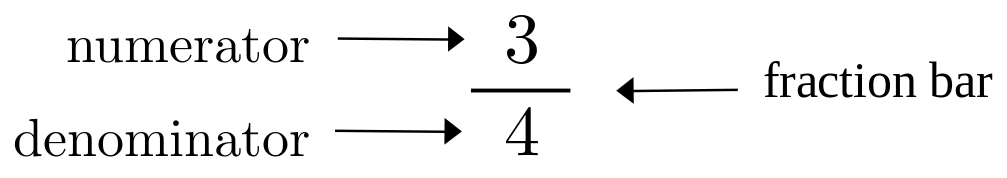
\includegraphics[width=0.7\textwidth]{fraction diagram.png}
\vspace{14pt}
\begin{center}
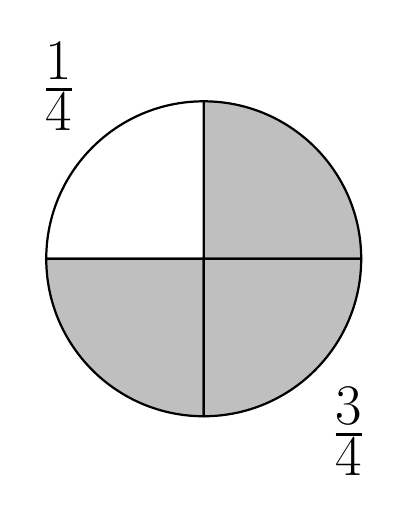
\begin{tikzpicture}
  \pie[
    color={lightgray, white, lightgray, lightgray},
    radius=2,
    before number=\phantom,
    after number=,
    sum=auto
    ]{25/{}, 25/{\fontsize{30}{34}\selectfont $\frac{1}{4}$}, 25/{}, 25/{\fontsize{30}{34}\selectfont $\frac{3}{4}$}}
\end{tikzpicture}
\end{center}

\section{Equivalent fractions}

\subsection*{Equivalent}
Equivalent means the same as or just as good as. Coke and Pepsi are equivalent drinks. They taste the nearly same so it doesn’t matter which one you get.

\item What does equivalent mean, in your own words?
\item Use equivalent in a sentence.

In maths, things are equivalent if they are different ways of writing the same amount. $3+3$ is equivalent to $2 \times 3$.\\

\item What does equivalent mean in maths, in your own words?
\item Think of two things in maths that are equivalent.

\subsubsection*{Express} When you have an idea it starts in your mind. For someone else to know what that idea is, you have to put the idea into the real world so that it can be heard or seen. Talking and writing are ways of expressing ideas to others. There are many ways to express ideas.\\

\item What does express mean, in your own words?
\item Think of an idea and think of two different ways of expressing that same idea.\\

In maths, express means to put a maths idea into maths symbols that others can read. $3 \times 4 + 2$ is an idea expressed in maths. Its like using words in a sentence but you are using the numbers and symbols of maths.\\

\item What does express mean in maths, in your own words?
\item Use express in a sentence that show this meaning.

\subsection*{Equivalent fractions}
Equivalent fractions are where you express the same amount in different ways. One half, $\frac{1}{2}$, two quarters, $\frac{2}{4}$, and four eighths, $\frac{4}{8}$ all express the same amount even though they have different numerators and denominators. They are called equivalent fractions.\\

\begin{tikzpicture}
  \pie[
    color={lightgray, white},
    hide number,
    radius=2,
    scale font={\fontsize{20}{24}\selectfont},
  ]{50/{$\frac{1}{2}$}, 50/{$\frac{1}{2}$}}

\pie[
    color={lightgray, lightgray, white, white},
    hide number,
    radius=2,
    pos={5.5,0},
    scale font={\fontsize{20}{24}\selectfont}
    ]{25/$\frac{1}{4}$, 25/$\frac{1}{4}$, 25/$\frac{1}{4}$, 25/$\frac{1}{4}$}

\pie[
    color={lightgray, lightgray, lightgray, lightgray, white, white, white, white},
    hide number,
    radius=2,
    pos={11.5,0},
    scale font={\fontsize{20}{24}\selectfont}
    ]{12.5/$\frac{1}{8}$, 12.5/$\frac{1}{8}$, 12.5/$\frac{1}{8}$, 12.5/$\frac{1}{8}$, 12.5/$\frac{1}{8}$, 12.5/$\frac{1}{8}$, 12.5/$\frac{1}{8}$, 12.5/$\frac{1}{8}$}

\end{tikzpicture}

\vspace{14pt}
Half of something, $\frac{1}{2}$, is the same amount as two quarters of it, $\frac{2}{4}$, and its also the same as four eighths, $\frac{4}{8}$. They are equivalent fractions.\\

\item What are equivalent fractions, in your own words?
\item Think of two fractions that are equivalent.

\subsection*{Making equivalent fractions}

To make equivalent fractions you multiply or divide both the numerator and denominator by the same number. The amount that the fraction expresses does not change as long as you do the same thing to both the top and the bottom of a fraction.

If you have the fraction $\frac{2}{4}$, you can multiply both the numerator and denominator by 2 to get the equivalent fraction $\frac{4}{8}$. You can divide both the numerator and denominator by 2 to get the equivalent fraction $\frac{1}{2}$.
$$\frac{2}{4} = \frac{2 \times 2}{4 \times 2} = \frac{4}{8}$$
$$\frac{2}{4} = \frac{2 \div 2}{4 \div 2} = \frac{1}{2}$$

\item What are 3 fractions that are equivalent to $\frac{2}{3}$?

\section{Simplifying fractions}

\subsection*{Simplify} Simplify means to make something simple so that it's easier.

\item What does simplify mean?
\item Use simplify in a sentence.\\

A fraction is easier to work with when it has been simplified. You do that by changing it into an equivalent fraction that has smaller numbers in it. When you simplify $\frac{4}{8}$ it becomes $\frac{1}{2}$.\\

\item What does it mean to simplify a fraction?
\item Use simplify in a sentence that show this meaning.

\subsection*{Greatest} In English, greatest means the best, as in a circus where they say its the Greatest Show on Earth. Greatest also meant biggest, like when you say things like my greatest fear is spiders.

\item What does greatest mean?
\item Use greatest in a sentence that shows its meaning as the biggest or the best.\\

In maths, greatest means the biggest number, like if you compare between 9 and 7, and say that 9 is the greatest.\\

\item What does greatest mean when it's a number?
\item Use greatest in a sentence that shows this meaning.

\subsection*{Common} Common means shared by two or more people or things, like when people share something in common.

\item What does common mean?
\item Use common in a sentence that shows its meaning as something shared.\\

In maths common means that two things have the same number in them somewhere. If you had two groups of numbers you would say that the common numbers were the ones that were in both groups. Say 2, 3, 4, 5 and 4, 5, 6, 7. The common numbers are 4 and 5.

\item What does common mean in maths?
\item What are the common numbers in 12,13,14,15 and 10, 11, 12, 13?

\subsection*{Factor} In English, a factor means a part of the cause for something. People might talk about the factors of some situation, meaning the different parts of it, time or money or the people involved.

\item What is a factor?
\item Use factor in a sentence that shows its meaning as a part of something.\\

In maths, factors are the numbers which will multiply to give some other number. For example, the factors of 8 are 1, 2, 4 and 8, because 1 $\times$ 8, 2 $\times$ 4, 4 $\times$ 2, and 8 $\times$ 1 all equal 8.

\item What is a factor, in maths?
\item What are some of the factors of 12?

\subsubsection*{Finding factors}
Divide the number by each counting number, in order. The pairs of factors are the divisors and the quotients where the quotient is a counting number. Continue only until the quotient is smaller than the divisor. Going past that point just results in the same factors but in reverse order. 

For example, to find the factors of 15:

\begin{doublespace}
$15 \div 1 = 15$\ \ \leftarrow\\
$15 \div 2 = 7 \frac{1}{2}$\\
$15 \div 3 = 5$\ \ \leftarrow\\
$15 \div 4 = 3 \frac{3}{4}$\ \ (quotient smaller than divisor)
\end{doublespace}

The pairs of factors of 15 here are 1 \&  15, and 3 \& 5, so the factors of 15 are 1, 3, 5 and 15.\\

\item What are the factors of 8?
\item What are the factors of 24?

\subsection*{Greatest Common Factor}
The largest number that has both the numerator and denominator of a fraction as a multiple is called the greatest common factor.\\

It is sometimes written just as GCF.\\

To simplify a fraction you divide the numerator and the denominator  by their greatest common factor.\\

\item In your own words, what does greatest common factor mean?
\item What is the purpose of finding the greatest common factor?
\item How is the greatest common factor of the numerator and denominator of a fraction used to simplify the fraction?\\

Simplified fractions are easier to work with. Always simplify a fraction if you can, both before you try to add, subtract, multiply or divide them, and in writing your final answer.

\item Why is it a good idea to simplify fractions?
\item Can $\frac{3}{6}$ be simplified?
\item What should you do if you worked out an answer that was $\frac{2}{4}$?

\subsubsection*{Cancelling}
To cancel something means to cross it out.\\

\item What does cancel mean?
\item Use cancel in a sentence.\\

To cancel a fraction means to divide the numerator and the denominator by their greatest common factor and cross them out and replace them. That is the easiest and usual way to write it when you simplify a fraction.\\

For $\frac{4}{8}$, the largest number that divides evenly into both the numerator and denominator is 4, but you don't bother to write that. You just cross out the 4 and write a 1, and cross out the 8 and write a 2. That gives you the equivalent simplified fraction of 1/2.

$$\text{So instead of writing }\frac{4}{8} = \frac{4 \div 4}{8 \div 4} = \frac{1}{2}\text{, you just write }\frac{4}{8} = \frac{^1 \cancel{4}}{\cancel{8}_2}\text{.}$$

\item What does cancelling a fraction mean?
\item Why do we cancel a fraction this way instead of writing what we are doing in full?
\item Simplify $\frac{6}{12}$ by cancelling.

\subsection*{How to Find the Greatest Common Factor}

\subsubsection*{Knowing the times table} You can often just simplify fractions in your head, if you know the times table well. With practice you can get good enough that you will know the greatest common factor right away without having to think much about it.\\

For example, maybe you can see that the greatest common factor needed to simplify $\frac{3}{9}$ is 3.
$$\frac{3}{9} = \frac{3 \div 3}{9 \div 3} = \frac{1}{3} \text{   or by cancelling you write }\frac{^1\cancel{3}}{\cancel{9}_3} = \frac{1}{3}$$

\item Using your knowledge of the times table, simplify 7/21.

\subsubsection*{Simplifying in stages} If you can't spot the greatest common factor right away, it will still work if you find just any common factor and use that to start with.\\

If the numerator and denominator are both even then you can at least divide them both by 2.\\

You will get a simpler fraction and then you can look at that one for a new common factor. Keep going until you are sure there are no more common factors.\\

Say you have to simplify $\frac{63}{84}$, and you spot that 3 divides evenly into both 63 and 84. You cancel both numbers and replace them.

$$\frac{^{21}\cancel{63}}{\cancel{84}_{28}}$$

Now you have $\frac{21}{28}$ and you see that 21 and 28 are multiples of 7, so you cancel both numbers again and replace them.

$$\frac{63}{84} = \frac{^{21}\cancel{63}}{\cancel{84}_{28}} = \frac{^3\cancel{21}}{\cancel{28}_4} = \frac{3}{4}$$

\item In stages, simplify $\frac{66}{198}.

\subsubsection*{Listing out all the factors}
You can also work out the factors and write them down to pick the greatest common factor. You’ll definitely get a right answer that way.

\vspace{28pt}
For example, to simplify $\frac{63}{105}$,

\vspace{28pt}
factors of 63: 1, 3, \textcircled{7,} 9, 21, 63

factors of 105: 1, 3, 5, \textcircled{7,} 15, 21, 35, 105

\vspace{28pt}
The greatest common factor of 63 and 105 is 7.

$$63 = \div 7 = 9 \text{ and }105 \div 7 = 15\text{, so }\frac{63}{105} = \frac{9}{15}$$

$$\text{You would write it as }\frac{^9 \cancel{63}}{\cancel{105}_{15}}$$

\vspace{28pt}
\item List out the factors and simplify these fractions: $\frac{14}{126}, \frac{8}{144}, \frac{21}{105}$.

\subsection*{Using Prime Factors to Simplify Fractions}
A foolproof way to simplify fractions is to find the prime factors of the numerator and denominator and rewrite the fraction as their product. Doing that can be easier than finding the greatest common factor when the numbers in the fraction get too big.

Remember prime factor trees? Any number that isn't a prime number can be expressed as a product of its prime factors.\\

To simplify $\frac{36}{48}$,
\begin{figure}[ht]
  \centering
  \begin{minipage}{0.4\textwidth}
    \centering
    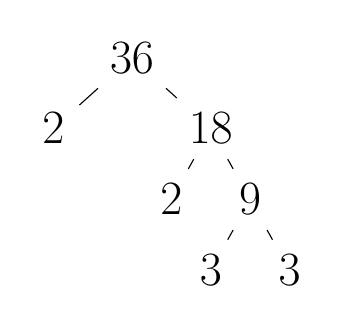
\begin{tikzpicture}[level distance=0.9cm,
      level 1/.style={sibling distance=2cm},
      level 2/.style={sibling distance=1cm}]
      \node {36}
        child {node {2}}
        child {node {18}
          child {node{2}}
          child {node {9}
            child {node {3}}
            child {node {3}}}
        };
    \end{tikzpicture}
\caption*{\hspace{1cm}$36 = 2 \times 2 \times 3 \times 3$}
    \label{fig:tree36}
  \end{minipage}%
  \hfill
  \begin{minipage}{0.4\textwidth}
    \centering
    \begin{tikzpicture}[level distance=0.9cm,
      level 1/.style={sibling distance=2cm},
      level 2/.style={sibling distance=1cm}]
      \node {48}
        child {node {2}}
        child {node {24}
          child {node{2}}
          child {node {12}
            child {node {2}}
            child {node {6}
              child {node {2}}
              child {node {3}}}
        }};
    \end{tikzpicture}
    \caption*{\hspace{1cm}$48 = 2 \times 2 \times2 \times 2 \times 3$}
    \label{fig:tree48}
  \end{minipage}
\end{figure}

$$\frac{36}{48} &= \frac{2 \times 2 \times 3 \times 3}{2 \times 2 \times2 \times 2 \times \times 3}$$\\

Now it's easy to see what to cancel.

$$\frac{36}{48} = \frac{{^1\cancel{2 \times 2}} \times 3 \times ^1{\cancel{3}}}{^1{\cancel{2 \times 2}} \times2 \times 2 \times \times {\cancel{3}}_1} = \frac{1 \times 3 \times 1}{1 \times 2 \times 2 \times 1} = \frac{3}{4}$$\\

\item Using prime factor trees and writing the denominator and numerator as products of prime numbers, simplify $\frac{84}{144}$, $\frac{48}{80}$, and $\frac{63}{127}$.

\section{Proper fractions \\and Improper fractions}

\subsection*{Proper} In English, proper mean that something is done right. Having proper manners means that you are doing the right thing.

\item What does proper mean, in your own words?
\item Use proper in a sentence.

Fraction means equal parts of a whole thing. It means less than 1 of something and not the whole thing. A fraction is proper when the numerator is smaller than the denominator, meaning that the fraction is less than 1. $\frac{3}{4}$ is a proper fraction.

\item What is a proper fraction?
\item Why do you think that fractions with the numerator smaller than the denominator are called proper fractions?
\item Give an example of a proper fraction.

\subsection*{Improper} Improper means that something is not being done right. Improper behaviour means bad conduct or being rude.

\item What does improper mean, in your own words?
\item Use improper in a sentence.

An improper fraction is one where the numerator is bigger than the denominator, so that the value of the fraction is greater than 1. It's not just an equal part of something so it's not properly a fraction. It's some value expressed as a fraction but it's not really a fraction, so it's called an improper fraction.

For example, $\frac{3}{2}$ means that you have 3 halves of something, an improper fraction, just like $\frac{13}{7}$ is also an improper fraction.

\item What is an improper fraction?
\item Why are fractions with the numerator larger than the denominator called improper fractions?
\item Give an example of an improper fraction.

\subsection*{Changing a whole number \\ into an improper fraction}
When you have a problem that involves both whole numbers and fractions, you the first step to solving it is to express the whole number as a fraction. That’s done by writing the whole number as the numerator and using a denominator of 1.

That works because fractions and dividing are similar things. $\frac{1}{2}$ is just another way of expressing $1 \div 2$. Any number divided by 1 doesn't change the number, so a fraction with a denominator of 1 means the same as dividing the numerator by 1, so the fraction still has the same overall value as just its numerator.\\

For example, $236 = 236 \div 1 = \frac{236}{1}$.\\

You can change any whole number into an improper fraction just by writing it as a fraction with a denominator of 1.\\

\item Pick 5 whole numbers and change them into improper fractions.

\section{Mixed fractions}

Mixed means that two or more things have been put together. You might hear of a dog being a mixed breed. A labradoodle is a mix of labrador and poodle.

\item What does mixed mean, in your own words?
\item Use mixed in a sentence.

A fraction that is a mix of a whole number plus a proper fraction is called a mixed fraction.

$1\frac{3}{4}$ is really saying $1 + \frac{3}{4}$, so it is a mixed fraction.

\item What is a mixed fraction, in your own words?
\item What is an example of a mixed freaction?

As well as simplifying a fraction if you can, you also change an improper fraction to a mixed fraction when you are writing your final answer.

\subsection*{Changing an improper fraction \\into a mixed fraction}
An improper fraction is greater than 1, so it's really a whole number plus a proper fraction.

To change an improper fraction to a mixed fraction you divide the numerator by the denominator. The result is the whole number part and the remainder is the numerator of the fraction part.\\

For example, $\frac{22}{7}$:

22 $\div$ 7 = 3, with a remainder of 1.

So $\frac{22}{7}$ = $3 \frac{1}{7}$.\\

\item What is the improper fraction $\frac{3}{2}$ as a mixed fraction?
\item What is the improper fraction $\frac{14}{5}$ as a mixed fraction?
\item What is the improper fraction $\frac{5}{3}$ as a mixed fraction?

\subsection*{Changing a mixed fraction \\ into an improper fraction}
Sometimes you have to change a mixed fraction back into an improper fraction. To do that you split the mixed fraction into the whole number part and the fraction part. Then you change the whole number part into an improper fraction and add the two fractions.

To find the numerator of the whole number part, multiply the whole number and the denominator of the fraction part.

The denominator of the whole number part is the same denominator as the fraction part.

\begin{align*}
\textrm{mixed fraction} &= \textrm{whole number}\ +\ \frac{\textrm{numerator}}{\textrm{denominator}}\\\\
&= \frac{\textrm{whole number}\ \times\ \textrm{denominator}}{\textrm{denominator}}\
+\ \frac{\textrm{numerator}}{\textrm{denominator}}
\end{align*}

\begin{align*}
\textrm{For example,}\ 2 \frac{3}{5} &= 2 + \frac{3}{5}\\
&= \frac{10}{5} + \frac{3}{5}\ = \frac{13}{5}
\end{align*}

\item What is the mixed fraction $1 \frac{1}{3}$ as an improper fraction?
\item What is the mixed fraction $2 \frac{1}{8}$ as an improper fraction?
\item What is the mixed fraction $1 \frac{4}{7}$ as an improper fraction?

\section{Multiplying fractions}
Multiplying two fractions is easy. You just multiply the two numerators and the two denominators and that’s your answer.

For example, $\frac{3}{7} \times \frac{5}{9} = \frac{15}{63}$.

And simplify your answer, of course: $\frac{^5\cancel{15}}{\cancel{63}_{21}} = \frac{5}{21}$.\\

\item What is $\frac{3}{4} \times \frac{2}{3}$?
\item What is $\frac{4}{5} \times \frac{7}{8}$?
\item What is $\frac{2}{7} \times \frac{1}{8}$?

\paragraph{of}
In word problems, the word "of" means "times." Things such as "seven eighths of fifteen" are solved by doing $\frac{7}{8}\times15=\frac{105}{8}=13\frac{1}{8}$.\\

\item What is half of $\frac{3}{4}$?
\item What is $\frac{2}{3}$ of 11?
\item What is $\frac{7}{8}$ of $\frac{5}{6}$?

\subsection*{Simplifying before Multiplying}
It is easier to simplify fractions before multiplying because the numbers will be smaller, and the answer will already be simplified.

$$\frac{9}{15} \times \frac{3}{9} =
\frac{{^3\cancel{9}}}{{\cancel{15}_5}} \times \frac{{^1\cancel{3}}}{{\cancel{9}_3}} = \frac{3\times1}{5\times3} = \frac{1}{15}$$

\item Simplify and multiply: $\frac{6}{8}\times\frac{3}{9}.$
\item Simplify and multiply: $\frac{12}{15}\times\frac{8}{18}.$
\item Simplify and multiply: $\frac{4}{12}\times\frac{12}{15}.$

\subsubsection*{Cross-Cancelling}
Because the order doesn't matter when you multiply, you can cancel either denominator with either numerator.

$$\frac{3}{10} \times \frac{2}{5} = \frac{{3 \times 2}}{{10 \times 5}} = \frac{{2 \times 3}}{{10 \times 5}} = \frac{2}{10} \times \frac{3}{5}$$

$$\text{That's why you can do }\frac{3}{{\cancel{10}_5}} \times \frac{{^1\cancel{2}}}{5} = \frac{3}{5} \times \frac{1}{5} = \frac{3}{25}\text{.}$$

You can also do this with any number of fractions.

$$\frac{4}{5} \times \frac{3}{4} \times \frac{2}{3} = \frac{{^1\cancel{4}}}{5} \times \frac{{^1\cancel{3}}}{{\cancel{4}_1}} \times \frac{2}{{\cancel{3}_1}} = \frac{1 \times 1 \times2}{5 \times 1 \times 1} = \frac{2}{5}$$

\item Cross-cancel and multiply: $\frac{9}{10} \times \frac{2}{3}$
\item Cross-cancel and multiply: $\frac{16}{15} \times \frac{21}{24}$
\item Cross-cancel and multiply: $\frac{2}{7} \times \frac{35}{6}$

\subsection*{Multiplying Mixed Fractions}
There are a few different ways that you can go about multiplying mixed fractions.\\

\subsubsection*{Converting to Improper Fractions}
To multiply mixed fractions, convert any mixed fraction to an improper fraction before you do the multiplication.\\

For example, $1 \frac{1}{3} \times 2 \frac{1}{4}:$

$$1 \frac{1}{3} = \frac{3}{3} + \frac{1}{3} = \frac{4}{3}$$
$$2 \frac{1}{4} = \frac{8}{4} + \frac{1}{4} = \frac{9}{4}$$
$$\frac{4}{3} \times \frac{9}{4} = \frac{^3 \cancel{36}}{\cancel{12}_1} = \frac{3}{1} = 3$$

\item Convert mixed fractions to improper fractions\\ and multiply: $2 \frac{2}{3} \times1 \frac{5}{7}$

\subsubsection*{Making Mixed Fractions Whole Numbers}
A fraction multiplied by its denominator becomes a whole number, which is easier to multiply. If you then also divide by the same amount, the overall product is unchanged.

\begin{align*}
36 \times 3 \frac{1}{2} &= 36 \times 3 \frac{1}{2} \times 2 \div 2\\
&= 36 \div 2 \times 3 \frac{1}{2} \times 2\\
&= 18 \times 7 = 126
\end{align*}

\item Convert fractions to whole numbers\\ and multiply: $3\frac{1}{3}\times4$.

\subsubsection*{Making Mixed Fractions Mixed Decimal Fractions}
Another way is to convert mixed fractions to a decimal fractions.\\
\begin{figure}[ht]
\begin{minipage}[b]{0.5\linewidth} \centering 
36 \times 3 \frac{1}{2} =
\end{minipage}
\begin{minipage}[b]{0.5\linewidth} \centering 
\begin{tabular}{c@{\,}c@{\,}c@{\,}c@{\,}c@{\,}c}
       & &3&6&.&0 \\
\times &_{1}&_{3} &3&.&5 \\
\hline
    &^{1}&1&8&0&0 \\
     + &1&0&8&0&0 \\
\hline
      1&2&6&.&0&0 \\
\hline
\hline
\end{tabular}\\
\end{minipage}\end{figure}\\

The decimal point is placed at the total number of fractional digits of the factors being mutliplied.\\

\item Convert $2\frac{1}{2}$ to a decimal fraction and multiply by 3.

\section{Dividing fractions}

\paragraph{Reciprocal}
Reciprocal means existing on both sides. For example, Australia has a reciprocal agreement with China to receive steel in exchange for iron ore.

\item What does reciprocal mean?
\item What is an example of something else that is reciprocal?

\paragraph{Reciprocal of a fraction}
The flipped version of a fraction is called its reciprocal. $\frac{2}{1}$ is the reciprocal of $\frac{1}{2}$\\

\item What does the reciprocal of a fraction mean?
\item What is the reciprocal of $\frac{3}{4}$?

\paragraph{How to divide fractions}
Dividing fractions is easy. You just have to flip one of the fractions first, to get its reciprocal, and then just multiply them.\\

For example,
$$\frac{3}{7} \div \frac{5}{9} = \frac{3}{7} \times \frac{9}{5} = \frac{27}{35}$$

Another example:

$$\frac{2}{3} \div \frac{5}{6} = \frac{2}{3} \times \frac{6}{5} = \frac{^4\cancel{12}}{\cancel{15}_5} = \frac{4}{5}$$

\item What is $\frac{3}{4} \div \frac{2}{3}$?
\item What is $\frac{3}{8} \div \frac{5}{9}$?
\item What is $\frac{2}{7} \div \frac{1}{6}$?

\subsection*{Dividing mixed fractions}
Convert mixed fractions to improper fractions first, do the division, simplify, and then convert the answer back to a mixed fraction.

For example, divide $8 \frac{1}{3}$ by 3 :

First convert both numbers to improper fractions:

$$8\frac{1}{3} \div 3 = \frac{24}{3} + \frac{1}{3} \div \frac{3}{1} = \frac{25}{3} \div \frac{3}{1}$$

Flip one of the fractions, and multiply:

$$\frac{25}{3} \div \frac{3}{1} = \frac{25}{3} \times \frac{1}{3} = \frac{25}{9}$$

Then convert the answer back to a proper fraction:

$$\frac{25}{9} = 2 \frac{7}{9}$$

\item What is $1 \frac{1}{2} \div 4$?
\item What is $3 \div \frac{2}{3}$?
\item What is $3 \frac{1}{4} \div 2 \frac{2}{5}$?

\section{Fractions\\with different denominators}
Adding or subtracting two fractions that have different denominators is harder than multiplying or dividing them. You can't just add the numerators or you'll get a wrong answer. Also comparing fractions to see which is the bigger or smaller can’t really be done with fractions that have different denominators. You’d just be guessing. The parts that you are adding or subtracting or comparing all have to be the same size or your answer won’t be right.

To add or subtract or compare two fractions with different denominators, you have to change both fractions into equivalent fractions that both have the same denominator.

Common means shared by both people or things, like when two people have something in common, so finding the denominator that both fractions can be changed into is called finding the common denominator. There are a few different ways of doing it.

When both fractions have been converted into equivalent fractions with a common denominator, then you can add or subtract the numerators and you’ll get a right answer.\\

\begin{tikzpicture}
  \pie[
    color={white, white, white, lightgray, lightgray, lightgray},
    hide number,
    radius=1.5,
    scale font={\fontsize{20}{24}\selectfont},
  ]{16.66/{}, 16.66/{}, 16.66/{}, 16.66/{}, 16.66/{}, 16.66/{$\frac{1}{2}$}}

\pie[
    color={white, white, white, white, lightgray, lightgray},
    hide number,
    radius=1.5,
    pos={6,0},
    scale font={\fontsize{20}{24}\selectfont}
    ]{16.66/{}, 16.66/{}, 16.66/{}, 16.66/{}, 16.66/{}, 16.66/{$+\ \frac{1}{3}$}}

\pie[
    color={white, lightgray, lightgray, lightgray, lightgray, lightgray},
    hide number,
    radius=1.5,
    pos={12,0},
    scale font={\fontsize{20}{24}\selectfont}
    ]{16.66/{}, 16.66/{}, 16.66/{}, 16.66/{}, 16.66/{}, 16.66/{$=\ \frac{5}{6}$}}
\end{tikzpicture}

$$\frac{1}{2} + \frac{1}{3} = \frac{3}{6} + \frac{2}{6} = \frac{5}{6}$$

\subsection*{Using 1 as a fraction\\to make equivalent fractions}
Fractions and dividing are similar things.

$\frac{3}{4}$ means the same as 3 $\div$ 4.

Also, any number divided by itself is equal to 1.

That means that you can express 1 as a fraction by having the numerator and denominator being both the same number. That's the same as dividing a number by itself, which will always equal 1.

$$\frac{3}{3} = \frac{1}{1} = \frac{123}{123} = \frac{12345}{12345} = \frac{17}{17} = 1$$

All of these fractions are just different ways of saying 1. You change a fraction into an equivalent fraction by multiplying the top and bottom numbers by the same amount. The reason that works is that you are really just multiplying the fraction by 1.

$$\frac{3}{4} \times \frac{3}{3} = \frac{9}{12}$$

You can convert a fraction to any equivalent fraction that you need by multiplying it by a 1 that has been expressed as a fraction.\\

Say you can have $\frac{1}{4}$ of a pizza but it's already been cut into 12 slices. How many twelfths of the pizza are you allowed to have?

Convert quarters to twelfths by multiplying by $\frac{3}{3}:$\\
$$\frac{1}{4}=\frac{1}{4}\times\frac{3}{3}=\frac{3}{12}.$$
So $\frac{1}{4}$ of a pizza = $\frac{3}{12}$ of a pizza or 3 slices.\\

\item Convert $\frac{3}{5}$ into tenths.
\item Convert $\frac{3}{8}$ into sixteenths.
\item Convert $\frac{1}{3}$ into twelfths.

\section{Comparing fractions}
Comparing two fractions with different denominators isn’t easy.

Which is bigger: $\frac{2}{3}$ or $\frac{3}{5}$ ? You can only really tell once you have converted them into equivalent fractions with the same denominators.

Once you work out that $\frac{2}{3} = \frac{10}{15}$ and $\frac{3}{5} = \frac{9}{15}$, then you can easily see that the answer is $\frac{2}{3}$.

\item Compare $\frac{1}{2}$ and $\frac{5}{8}$. Which is bigger?

\subsection*{Cross-multiplying}
A shortcut to comparing fractions, so that you don't have to convert them to equivalent fractions, is cross-multiplying. That means multiplying the numerator of one fraction by the denominator of the other fraction. Then you can properly compare.

\begin{doublespace}
For example, comparing $\frac{2}{3}$ and $\frac{3}{5}$:

$2 \times 5 = 10$ and $3 \times 3 = 9$,

so $\frac{2}{3}$ is greater than $\frac{3}{5}$.
\end{doublespace}

\item Cross-multiply and compare $\frac{5}{7}$ and $\frac{6}{11}$. Which is bigger?

\section{Adding and Subtracting fractions}
\paragraph{Adding and Subtracting fractions with the same denominator}
Adding and subtracting two fractions with the same denominator is easy. Add or subtract their numerators and write the result over the denominator.

$$\text{For example, }\frac{1}{4} + \frac{2}{4} = \frac{3}{4}\text{, and }\frac{2}{3} - \frac{1}{3} = \frac{1}{3}$$

\item What is $\frac{3}{9}+\frac{4}{9}$?\\

\paragraph{Adding and Subtracting fractions with different denominators}
You can't just add or subtract the numerators of fractions that have different denominators, though. You'll get a wrong answer.

You can't take pizzas that have been cut into thirds and pizzas that have been cut into quarters and just hand out pieces as if they were all the same size. You have to cut both pizzas the right amount so that all the pieces of both pizzas are the same size first.

Before you can add or subtract fractions that have different denominators, you have to change them into equivalent fractions that both have the same denominator.

\subsection*{Common Denominator}
You need to find a number to multiply the top and bottom of each fraction by that will give both fractions the same denominator. That's called finding the common denominator. When you have that, you can change them into fractions with a common denominator.


\subsection*{Finding the common denominator}

\subsubsection*{Multiply the denominators}
The easiest way to find a common denominator is to just multiply the two denominators.\\

For example, $\frac{1}{3} + \frac{1}{4}$.

Common denominator: $3 \times 4 = 12$.

Then multiply both fractions to convert them to equivalent fractions with this common denominator.

$$\frac{1}{3} + \frac{1}{4} = (\frac{1}{3} \times \frac{4}{4}) + (\frac{1}{4} \times \frac{3}{3}) = \frac{4}{12}+\frac{3}{12} = \frac{7}{12}$$

\subsection*{Lowest Common Denominator}
It's best to find the lowest common denominator and not just any multiple, so you are multiplying the easiest number possible.

The lowest common denominator is also called the lowest common multiple.\\

They are sometimes written just as LCD or LCM.\\

So if we were adding $\frac{1}{4} + \frac{1}{5}$:

Multiples of 4: 4, 8, 12, 16, \textcircled{20}

Multiples of 5: 5, 10, 15, \textcircled{20}, 25

The lowest common multiple is 12, so:
$$\frac{1}{4} + \frac{1}{5}
= (\frac{1}{4} \times \frac{5}{5})
+ (\frac{1}{5} \times \frac{4}{4})
= \frac{5}{20}+\frac{4}{20}
= \frac{9}{20}.$$

\subsubsection*{List the multiples of the denominators}
A thorough way to find common denominators is to list out the multiples of each denominator and pick the lowest number that is common to both lists.

\item Add $\frac{3}{7}$ and $\frac{2}{5}$ by listing the multiples of their denominators to find the lowest common denominator.

\subsubsection*{Finding which multiplier to use}
As covered earlier, equivalent fractions are made by using 1, expressed as a fraction, as a multiplier.\\

To find just what multiplier is needed, divide the lowest common denominator by the denominator.\\

Say you have $\frac{1}{3}$ and $\frac{1}{4}$.

The lowest common denominator of 3 and 4 is 12.

The denominator of $\frac{1}{3}$ is 3.

$12 \div 3$ = 4, so multiply $\frac{1}{3}$ by $\frac{4}{4}$ to get $\frac{4}{12}$.

In the same way, $12 \div 4$ = 3, so multiply $\frac{1}{4}$ by $\frac{3}{3}$ to get $\frac{3}{12}$.

$$\frac{1}{3} + \frac{1}{4} = \frac{4}{12} + \frac{3}{12} = \frac{7}{12}.$$\\

Here is another example with subtraction:
$$\frac{3}{5} - \frac{1}{4}$$

Common denominator: $5 \times 4 = 20$.

$$\frac{20}{5} = 4\text{, so multiply }\frac{3}{5} \text{ by }\frac{4}{4}$$

$$\frac{20}{4} = 5\text{, so multiply }\frac{1}{4}\text{ by }\frac{5}{5}\text{ :}$$

$$\frac{3}{5} - \frac{1}{4} = \left(\frac{3}{5} \times \frac{4}{4}\right) - \left(\frac{1}{4} \times \frac{5}{5}\right) = \frac{12}{20} - \frac{5}{20} = \frac{7}{20}$$\\

\item What is $\frac{1}{2}+\frac{1}{7}$?
\item What is $\frac{2}{5}+\frac{3}{8}$?
\item What is $\frac{4}{9}+\frac{2}{5}$?
\item What is $\frac{3}{4}+\frac{4}{9}$?
\item What is $\frac{9}{11}+\frac{2}{7}$?

\subsection*{Cross-Multiplying}

A simple method to add and subtract fractions is cross-multiplying:
\begin{figure}[ht]
\begin{minipage}[ht]{0.4\linewidth} \centering
\begin{large}$\frac{2}{3}+\frac{1}{5}=$\end{large}\\
\vspace{8pt}
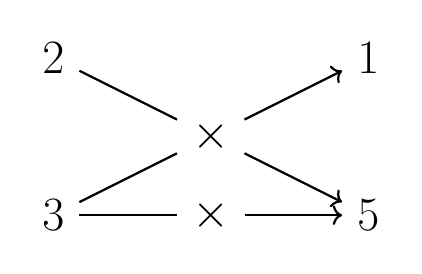
\begin{tikzpicture} 
\path ( 0, 0) node (times)   {$\times$};
\path (-2, 1) node (two)     {2};
\path ( 2, 1) node (one)     {1};
\path (-2,-1) node (three)   {3};
\path ( 2,-1) node (five)    {5};
\path ( 0,-1) node (timess)  {$\times$};
\draw [thick] (two) -- (times);
\draw [thick,->] (times) -- (five);
\draw [thick] (three) -- (times);
\draw [thick,->] (times) -- (one);
\draw [thick] (three) -- (timess);
\draw [thick,->] (timess) -- (five);
\end{tikzpicture}
\end{minipage}
\begin{minipage}[ht]{0.6\linewidth} \centering 
\begin{center}
\begin{align*}
&= \frac{(2 \times 5) + (3 \times 1)}{(3 \times 5)}\\\\
&= \frac{10+3}{15} = \frac{13}{15}
\end{align*}
\end{center}
\end{minipage}
\end{figure}

\item Using cross-multiplying, what is $\frac{2}{3}+\frac{2}{5}$?
\item Using cross-multiplying, what is $\frac{3}{4}+\frac{4}{7}$?
\item Using cross-multiplying, what is $\frac{4}{9}+\frac{1}{12}$?\\

Here is another example of cross multiplying to add fractions:
\begin{figure}[ht]
\begin{minipage}[ht]{0.4\linewidth} \centering
\begin{large}$\frac{3}{8}+\frac{2}{9}=$\end{large}\\
\vspace{8pt}
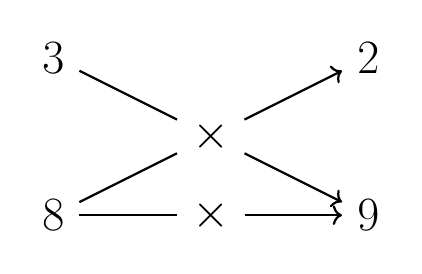
\begin{tikzpicture} 
\path ( 0, 0) node (times)   {$\times$};
\path (-2, 1) node (three)   {3};
\path ( 2, 1) node (two)     {2};
\path (-2,-1) node (eight)   {8};
\path ( 2,-1) node (nine)    {9};
\path ( 0,-1) node (timess)  {$\times$};
\draw [thick] (three) -- (times);
\draw [thick,->] (times) -- (nine);
\draw [thick] (eight) -- (times);
\draw [thick,->] (times) -- (two);
\draw [thick] (eight) -- (timess);
\draw [thick,->] (timess) -- (nine);
\end{tikzpicture}
\end{minipage}
\begin{minipage}[ht]{0.6\linewidth} \centering 
\begin{center}
\begin{align*}
&=\frac{(3\times9)+(8\times2)}{(8\times9)}\\\\
&=\frac{27+16}{72}=\frac{43}{72}.\\
\end{align*}
\end{center}
\end{minipage}
\end{figure}

\end{enumerate}

\section*{Congratulations!}

\textbf{You have mastered fractions.}\\

Now review any parts of this course that you are unsure of, and then work your way through these final questions:

\section*{Questions:}

\begin{enumerate}
\item Compare $\frac{1}{3}$ and $\frac{2}{5}$.
\item Add $\frac{3}{4}$ and $\frac{1}{8}$.
\item Subtract $\frac{5}{6}$ from $\frac{2}{3}$.
\item Multiply $\frac{2}{3}$ and $\frac{4}{5}$.
\item Divide $\frac{3}{4}$ by $\frac{2}{3}$.
\item Find an equivalent fraction for $\frac{1}{4}$ with a denominator of 12.
\item Simplify $\frac{6}{12}$.
\item Calculate $\frac{9}{15}$ in its simplest form.
\item Find the greatest common factor (GCF) of 24 and 36.
\item Determine the lowest common denominator for $\frac{1}{3}$ and $\frac{1}{4}$.
\item Add $\frac{2}{7}$ and $\frac{3}{7}$.
\item Subtract $\frac{5}{8}$ from $\frac{3}{8}$.
\item Multiply $\frac{2}{9}$ and $\frac{3}{4}$.
\item Divide $\frac{5}{6}$ by $\frac{1}{2}$.
\item Find an equivalent fraction for $\frac{3}{5}$ with a denominator of 20.
\item Simplify $\frac{12}{24}$.
\item Calculate $\frac{8}{10}$ in its simplest form.
\item Find the GCF of 18 and 27.
\item Determine the LCD for $\frac{1}{5}$ and $\frac{1}{6}$.
\item Add $\frac{1}{8}$ and $\frac{1}{16}$.
\item Subtract $\frac{5}{9}$ from $\frac{4}{9}$.
\item Multiply $\frac{2}{5}$ and $\frac{5}{7}$.
\item Divide $\frac{3}{4}$ by $\frac{2}{5}$.
\item Find an equivalent fraction for $\frac{2}{3}$ with a denominator of 9.
\item Simplify $\frac{15}{30}$.
\item Calculate $\frac{10}{20}$ in its simplest form.
\item Find the GCF of 36 and 48.
\item Determine the LCD for $\frac{2}{9}$ and $\frac{1}{6}$.
\item Add $\frac{1}{2}$ and $\frac{3}{4}$.
\item Subtract $\frac{5}{6}$ from $\frac{7}{8}$.
\item Multiply $\frac{1}{3}$ and $\frac{4}{9}$.
\item Divide $\frac{2}{5}$ by $\frac{3}{4}$.
\item Find an equivalent fraction for $\frac{5}{7}$ with a denominator of 35.
\item Simplify $\frac{20}{40}$.
\item Calculate $\frac{14}{28}$ in its simplest form.
\item Find the GCF of 42 and 56.
\item Determine the LCD for $\frac{3}{5}$ and $\frac{2}{3}$.
\item Add $\frac{4}{7}$ and $\frac{5}{7}$.
\item Subtract $\frac{9}{10}$ from $\frac{3}{10}$.
\item Multiply $\frac{3}{5}$ and $\frac{4}{7}$.
\item Divide $\frac{2}{3}$ by $\frac{1}{4}$.
\item Find an equivalent fraction for $\frac{4}{6}$ with a denominator of 12.
\item Simplify $\frac{16}{32}$.
\item Calculate $\frac{9}{18}$ in its simplest form.
\item Find the GCF of 30 and 45.
\item Determine the LCD for $\frac{2}{8}$ and $\frac{3}{12}$.
\item Add $\frac{1}{3}$ and $\frac{1}{6}$.
\item Subtract $\frac{7}{8}$ from $\frac{1}{8}$.
\item Multiply $\frac{3}{4}$ and $\frac{2}{3}$.
\item Divide $\frac{5}{6}$ by $\frac{2}{5}$.
\item Convert the mixed fraction $1\frac{3}{4}$ into an improper fraction.
\item Add $2\frac{2}{3}$ and $3\frac{1}{6}$.
\item Subtract $4\frac{3}{5}$ from $5\frac{4}{7}$.
\item Multiply $2\frac{1}{2}$ and $3\frac{2}{3}$.
\item Divide $6\frac{1}{4}$ by $2\frac{1}{2}$.
\item Convert the improper fraction $\frac{11}{4}$ into a mixed fraction.
\item Add $\frac{9}{2}$ and $3\frac{1}{3}$.
\item Subtract $\frac{7}{5}$ from $4\frac{3}{10}$.
\item Multiply $\frac{5}{8}$ and $2\frac{3}{4}$.
\item Divide $7\frac{2}{9}$ by $\frac{3}{4}$.
\end{enumerate}

\subsection*{Answers}

\begin{enumerate}
\item $\frac{1}{3} < \frac{2}{5}$
\item $\frac{3}{4} + \frac{1}{8} = \frac{7}{8}$
\item $\frac{2}{3} - \frac{5}{6} = \frac{1}{6}$
\item $\frac{2}{3} \cdot \frac{4}{5} = \frac{8}{15}$
\item $\frac{3}{4} \div \frac{2}{3} = \frac{9}{8}$
\item $\frac{1}{4}$ with a denominator of 12 is $\frac{3}{12}$
\item $\frac{6}{12} = \frac{1}{2}$
\item $\frac{9}{15} = \frac{3}{5}$
\item GCF of 24 and 36 is 12.
\item LCD for $\frac{1}{3}$ and $\frac{1}{4}$ is 12.
\item $\frac{2}{7} + \frac{3}{7} = \frac{5}{7}$
\item $\frac{3}{8} - \frac{5}{8} = -\frac{1}{8}$
\item $\frac{2}{9} \cdot \frac{3}{4} = \frac{1}{6}$
\item $\frac{5}{6} \div \frac{1}{2} = \frac{5}{3}$
\item $\frac{3}{5}$ with a denominator of 20 is \frac{12}{20}$
\item $\frac{12}{24} = \frac{1}{2}$
\item $\frac{8}{10} = \frac{4}{5}$
\item GCF of 18 and 27 is 9.
\item LCD for $\frac{1}{5}$ and $\frac{1}{6}$ is 30.
\item $\frac{1}{8} + \frac{1}{16} = \frac{3}{16}$
\item $\frac{4}{9} - \frac{5}{9} = -\frac{1}{9}$
\item $\frac{2}{5} \cdot \frac{5}{7} = \frac{2}{7}$
\item $\frac{3}{4} \div \frac{2}{5} = \frac{15}{8}$
\item $\frac{2}{3}$ with a denominator of 9 is $\frac{6}{9}$
\item $\frac{15}{30} = \frac{1}{2}$
\item $\frac{10}{20} = \frac{1}{2}$
\item GCF of 36 and 48 is 12.
\item LCD for $\frac{2}{9}$ and $\frac{1}{6}$ is 18.
\item $\frac{1}{2} + \frac{3}{4} = \frac{5}{4}$
\item $\frac{7}{8} - \frac{5}{6} = \frac{1}{24}$
\item $\frac{1}{3} \cdot \frac{4}{9} = \frac{4}{27}$
\item $\frac{2}{5} \div \frac{3}{4} = \frac{8}{15}$
\item $\frac{5}{7}$ with a denominator of 35 is \item \item $\frac{25}{35}$
\item $\frac{20}{40} = \frac{1}{2}$
\item $\frac{14}{28} = \frac{1}{2}$
\item GCF of 42 and 56 is 14.
\item LCD for $\frac{3}{5}$ and $\frac{2}{3}$ is 15.
\item $\frac{4}{7} + \frac{5}{7} = \frac{9}{7}$
\item $\frac{3}{10} - \frac{9}{10} = -\frac{6}{10}$
\item $\frac{3}{5} \cdot \frac{4}{7} = \frac{12}{35}$
\item $\frac{2}{3} \div \frac{1}{4} = \frac{8}{3}$
\item $\frac{4}{6}$ with a denominator of 12 is $\frac{8}{12}$
\item $\frac{16}{32} = \frac{1}{2}$
\item $\frac{9}{18} = \frac{1}{2}$
\item GCF of 30 and 45 is 15.
\item LCD for $\frac{2}{8}$ and $\frac{3}{12}$ is 12.
\item $\frac{1}{3} + \frac{1}{6} = \frac{1}{2}$
\item $\frac{1}{8} - \frac{7}{8} = -\frac{3}{4}$
\item $\frac{3}{4} \cdot \frac{2}{3} = \frac{1}{2}$
\item $\frac{5}{6} \div \frac{2}{5} = \frac{25}{12}$
\item $1\frac{3}{4}$ as an improper fraction is $\frac{7}{4}$.
\item $2\frac{2}{3} + 3\frac{1}{6} = 6\frac{1}{2}$.
\item $5\frac{4}{7} - 4\frac{3}{5} = 1\frac{25}{35}$ (simplified to $2\frac{5}{7}$).
\item $2\frac{1}{2} \cdot 3\frac{2}{3} = 7\frac{1}{6}$.
\item $6\frac{1}{4} \div 2\frac{1}{2} = 2\frac{1}{8}$.
\item $\frac{11}{4}$ as a mixed fraction is $2\frac{3}{4}$.
\item $\frac{9}{2} + 3\frac{1}{3} = 5\frac{2}{3}$.
\item $4\frac{3}{10} - \frac{7}{5} = 3\frac{1}{10}$.
\item $\frac{5}{8} \cdot 2\frac{3}{4} = 1\frac{11}{16}$.
\item $7\frac{2}{9} \div \frac{3}{4} = 9\frac{1}{3}$.
\end{enumerate}

\end{document}